\documentclass[aspectratio=169,9pt]{beamer}
\mode<presentation> 
\usepackage[utf8]{inputenc}
\usepackage{sansmathaccent} %Für equations
\usepackage{amsmath}
\usepackage{tikz}
\usepackage{multicol}
\usepackage{cancel}
\usepackage{relsize}
\usepackage[table]{xcolor}
\usepackage[labelfont={bf},font={color=black!40,footnotesize},tablename={Tabelle},figurename={Abbildung}]{caption}
\usetikzlibrary{positioning, arrows.meta, calc}
\usefonttheme[onlymath]{serif}
%\makeatletter
%\makeatother

\rowcolors{2}{miugray!30}{miugray!10}

\usetheme{Madrid}  %% Themenwahl
\useoutertheme{split} % Alternatively: miniframes, infolines, split
%\useinnertheme{circles}


\setbeamertemplate{itemize item}{\color{miugray}$\blacksquare$}
\setbeamertemplate{itemize subitem}{\color{uniblau}$\bullet$}



\newcommand{\metermilli}{\mskip3mu \text{mm}}
\newcommand{\cm}{\mskip3mu \text{cm}}
\newcommand{\m}{ \text{m}}
\newcommand{\lite}{ \text{l}}
\newcommand{\kg}{ \text{kg}}
\newcommand{\g}{ \text{g}}
\newcommand{\km}{ \text{km}}
\newcommand{\h}{ \text{h}}
\newcommand{\s}{ \text{s}}
\newcommand{\tonne}{ \text{t}}

\newcommand{\RA}{$\rightarrow$~}
\newcommand{\pp}{\par \vspace*{2mm}}
\newcommand{\ppbig}{\par \vspace*{4mm}}

\definecolor{miudiutex}{HTML}{1d2926}
\definecolor{miugray}{HTML}{b4cccf}
\definecolor{miugray2}{HTML}{4d7365}
\definecolor{white2}{HTML}{f5f7f8}
\definecolor{red}{HTML}{cf1f5c}
\definecolor{green}{HTML}{00A36C}
\definecolor{delphinidin}{HTML}{315794}
\definecolor{uniblau}{HTML}{004e9f}
\definecolor{unigelb}{HTML}{fcba00}
\definecolor{unigrau}{HTML}{909085}
\definecolor{pelargonidin}{HTML}{b33807}
\definecolor{cyanidin}{HTML}{ba0746}
\definecolor{paeonidin}{HTML}{d15ca6}
\definecolor{petunidin}{HTML}{b56fed}
\definecolor{malvidin}{HTML}{8a2d8c}

%\setbeamercolor{palette primary}{bg=pelargonidin!35,fg=white}
%\setbeamercolor{palette secondary}{bg=delphinidin!45,fg=white}
\setbeamercolor{palette primary}{bg=uniblau!70,fg=white}
\setbeamercolor{palette secondary}{bg=uniblau!45,fg=white}
\setbeamercolor{palette tertiary}{bg=unigelb!70,fg=unigrau}
\setbeamercolor{palette quaternary}{bg=miugray,fg=white}
\setbeamercolor{structure}{fg=black} % itemize, enumerate, etc
\setbeamercolor{section in toc}{fg=red} % TOC sections

\setbeamersize{text margin left=2cm,text margin right=2cm}


\useinnertheme{tcolorbox} 
\newcommand{\goodtk}[2]{
\begin{tcolorbox}[
	enhanced,
	colframe=uniblau!75,
	sharp corners,
	boxsep=5pt,
	title=\bfseries \sffamily #1,
	colback=white,
	coltitle=black,
	attach boxed title to top text left={yshift=-\tcboxedtitleheight/2},
	boxed title style={colback=white,colframe=white}
]
	#2
	\end{tcolorbox}
}
	
\newcommand{\antwort}[1]{
\begin{tcolorbox}[
	enhanced,
	colframe=unigrau!65,
	sharp corners,
	boxsep=1pt,
	colback=white,
	coltitle=black,
]
	#1
	\end{tcolorbox}
}


\title{2. Übung}
\author{PD Dr. Helene Loos}
\date{\today}

\begin{document}
%\maketitle
\small





\section{Organisatorisches}
\begin{frame}

\begin{center}

\Huge 
Übung 2
\pp
\small
Prozessbezogene Lebensmitteltechnologie
\end{center}

\end{frame}



\begin{frame}
\Large Wie läuft die Übung in Zukunft ab?
\pp
\normalsize
\begin{itemize}
\item Besprechungsteil (1. Hälfte $\sim$45 min):
\begin{itemize}

\item Freitags wird das Übungsblatt für die nächste Woche hochgeladen
\item Sie bereiten das Übungsblatt vor und rechnen die Aufgaben eigenständig
\item In der Übung werden die Aufgaben besprochen und Probleme geklärt
\item Lösungen werden zur Verfügung gestellt

\end{itemize}
\pp
\item Wiederholungsteil (2. Hälfte $\sim$45 min):
\begin{itemize}
\item Vorbereitung auf die Klausur
\item Es werden neue Aufgaben zu alten Themen zur Verfügung gestellt um das Gelernte zu vertiefen
\item Aufgaben und dazugehörige Lösungen werden \textbf{nicht} hochgeladen
\end{itemize}
\end{itemize}
\end{frame}

%\begin{frame}
%
%\begin{center}
%\begin{minipage}{.6\textwidth}
%\textbf{Nachtrag letzte Woche:}
%\begin{itemize}
%\item $\vartheta$ oder $\theta$ wird zwar für Grad Celsius verwendet, ist aber oft in Lehrbüchern trotzdem als $T$ angegeben
%\item Wie Wasseranteil in Klausur angeben? \RA Wird in der Aufgabenstellung klar kommuniziert
%\end{itemize}
%\end{minipage}
%\end{center}
%
%\end{frame}

\section{Aufgaben}
\begin{frame}

\begin{center}
Thema: \par 
\Huge 
Strömungen
\pp
\normalsize
von Fluiden und Gasen \par (ohne Reibung)
\end{center}

\end{frame}





\begin{frame}
\subsection*{Aufgabe 1}
\begin{minipage}{.5\textwidth}

\small
{\color{miugray}$\blacksquare ~$} \textbf{Aufgabe 1} \par \vspace*{2mm}

Ein Fluid durchströmt ein Rohr mit drei unterschiedlichen Querschnittsflächen. Im ersten Bereich
beträgt die Querschnittsfläche \textbf{20 cm$^2$} und die Fließgeschwindigkeit des Fluids beträgt \textbf{3 cm/s}.
\begin{itemize}
\item[a)] Im zweiten Bereich beträgt die Querschnittsfläche \textbf{10 cm$^2$}. Wie hoch ist die Geschwindigkeit des Fluids hier?
\item[b)] Im dritten Bereich beträgt die Querschnittsfläche \textbf{25 cm$^2$}. Wie hoch ist die Geschwindigkeit des Fluids hier?
\end{itemize}
\end{minipage}\hspace*{4mm}
\begin{minipage}{.5\textwidth}

\antwort{
\uncover<2->{
a) 
\begin{align*}
v_2 &= \frac{A_1}{A_2} \cdot v_1 \\
v_2 &= \frac{20~\text{cm}^2}{10~\text{cm}^2} \cdot 3~\text{cm/s} \\
	&= 6 ~\text{cm/s}
\end{align*}
}
\uncover<3->{
b)

\begin{align*}
v_2 &= \frac{A_1}{A_3} \cdot v_1 \\
v_3 &= \frac{20~\text{cm}^2}{25~\text{cm}^2} \cdot 3~\text{cm/s} \\
	&= 2,4 ~\text{cm/s}
\end{align*}
}
}
\end{minipage}



\end{frame}




\begin{frame}

\begin{minipage}{.5\textwidth}
\small
{\color{miugray}$\blacksquare ~$} \textbf{Aufgabe 2} \par \vspace*{2mm}

In einer Wasserstrahl-Vakuumpumpe, die wie ein Venturi-Rohr aufgebaut ist, fließen \mbox{4 L/min} Wasser. Der Durchmesser der Zuleitung (und Ableitung) beträgt \mbox{14 mm}, der Durchmesser an der engsten Stelle 3 mm. \par 
Der absolute Druck am Ausgang der Wasserstrahl-Vakuumpumpe entspricht einem Umgebungsdruck von 1 bar. Der geodätische Höhenunterschied kann vernachlässigt werden. \par  
Welcher relativer Unterdruck wird an der engsten Stelle erreicht? Welcher absolute Druck herrscht an der engsten Stelle?
\pp
\colorbox{unigelb}{\parbox{\textwidth}{\textbf{Hinweis:} Wir nehmen eine reibungsfreie Strömung an}}

\end{minipage}%
\hspace*{4mm}
\begin{minipage}{.5\textwidth}
\includegraphics[width=6cm]{F://LaTeX-Files/pngs/venturi2.pdf}


\small
\uncover<2->{Bernoulli:}
\begin{align*}
\only<2>{p_1 + \frac{\rho \cdot v_1^2}{2} + \rho g h_1 &= p_2 + \frac{\rho \cdot v_2^2}{2} \cdot \rho g h_2 \\}
\only<3>{p_1 + \frac{\rho \cdot v_1^2}{2} + \cancel{\rho g h_1} &= p_2 + \frac{\rho \cdot v_2^2}{2} \cdot \cancel{\rho g h_2} \\}
\only<4>{p_1 + \frac{\rho \cdot v_1^2}{2} &= p_2 + \frac{\rho \cdot v_2^2}{2}  \\}
\only<5>{p_1 + \frac{\rho \cdot \textcolor{uniblau}{\mathlarger{\mathlarger{v_1^2}}}}{2} &= p_2 + \frac{\rho \cdot \textcolor{uniblau}{ \mathlarger{\mathlarger{v_2^2}}}}{2}  \\}
\end{align*}

\end{minipage}%

\end{frame}


%\begin{frame}
%\begin{minipage}{.5\textwidth}
%
%
%\begin{align*}
%\dot{V} &= ~\text{const.} \\
%\dot{V} &= v \cdot A \qquad \rightarrow v = \frac{\dot{V}}{A} \\ \\
%v_1 &= \frac{\dot{V}}{A_1} \\
%	&= \frac{4~\text{L/min}}{\pi \cdot (0,007~\text{m})^2} \\
%	&= \frac{6,\overline{6} \cdot 10^{-5} ~\text{m$^3$}}{1,54 \cdot 10^{-4}~\text{m}^2 \cdot \text{s}} \\
%v_1 &= 0,43\mskip3mu \m/\text{s}
%\end{align*}
%\end{minipage}%
%\begin{minipage}{.5\textwidth}
%\includegraphics[width=7cm]{F://LaTeX-Files/pngs/venturi3a.pdf}
%\end{minipage}
%
%
%
%\end{frame}




\begin{frame}
\begin{minipage}{.5\textwidth}
\includegraphics[width=6cm]{F://LaTeX-Files/pngs/venturi2.pdf}


\small
Bernoulli:
\begin{align*}
p_1 + \frac{\rho \cdot \textcolor{uniblau}{v_1^2}}{2} &= p_2 + \frac{\rho \cdot \textcolor{uniblau}{v_2^2}}{2}
\end{align*}

\end{minipage}%
\hspace*{4mm}
\begin{minipage}{.5\textwidth}

\antwort{
\small
\begin{align*}
\uncover<2->{
\dot{V} &= ~\text{const.} \\}
\uncover<3->{
\dot{V} &= v \cdot A \qquad \rightarrow v = \frac{\dot{V}}{A} \\ \\}
\uncover<4->{
v_1 &= \frac{\dot{V}}{A_1} \\}
\uncover<5->{	&= \frac{4~\text{L/min}}{\pi \cdot (0,007~\text{m})^2} \\
	&= \frac{6,\overline{6} \cdot 10^{-5} ~\text{m$^3$}}{1,54 \cdot 10^{-4}~\text{m}^2 \cdot \text{s}} \\
v_1 &= 0,43\mskip3mu \m/\text{s}}
\end{align*}}
\end{minipage}%
\end{frame}





%\begin{frame}
%\begin{minipage}{.5\textwidth}
%
%
%\begin{align*}
%v_2 &= \frac{v_1 \cdot A_1}{A_2}\\
%&= v_1 \cdot \frac{A_1^2}{A_2^2} \\
%&= v_1 \cdot \frac{\cancel{\pi} \cdot \left( \frac{d_1}{\cancel{2}}\right)^2}{\cancel{\pi} \cdot \left( \frac{d_2}{\cancel{2}} \right)^2} \\
%&= v_1 \cdot \frac{d_1^2}{d_2^2} \\
%&= 0,43\mskip3mu \text{m/s} \cdot \frac{14^2}{3^2} \\
%&=9,36\mskip3mu \text{m/s}
%\end{align*}
%\end{minipage}%
%\begin{minipage}{.5\textwidth}
%\includegraphics[width=7cm]{F://LaTeX-Files/pngs/venturi3b.pdf}
%\end{minipage}
%
%
%
%\end{frame}

\begin{frame}
\begin{minipage}{.5\textwidth}
\includegraphics[width=6cm]{F://LaTeX-Files/pngs/venturi2.pdf}


\small
Bernoulli:
\begin{align*}
p_1 + \frac{\rho \cdot \textcolor{uniblau}{v_1^2}}{2} &= p_2 + \frac{\rho \cdot \textcolor{uniblau}{v_2^2}}{2}
\end{align*}

\end{minipage}%
\hspace*{4mm}
\begin{minipage}{.5\textwidth}

\antwort{
\small
\begin{align*}
v_2 &= \frac{v_1 \cdot A_1}{A_2}\\
\uncover<2->{&= v_1 \cdot \frac{A_1}{A_2} \\}
\uncover<3->{&= v_1 \cdot \frac{\alt<4->{\cancel{\pi}}{\pi} \cdot \left( \frac{d_1}{\alt<4->{\cancel{2}}{2}}\right)^2}{\alt<4->{\cancel{\pi}}{\pi} \cdot \left( \frac{d_2}{\alt<4->{\cancel{2}}{2}} \right)^2}\\}
\uncover<5->{&= v_1 \cdot \frac{d_1^2}{d_2^2} \\}
\uncover<6->{&= 0,43\mskip3mu \text{m/s} \cdot \frac{14^2}{3^2} \\}
\uncover<7->{&=9,36\mskip3mu \text{m/s}}
\end{align*}}
\end{minipage}%e 
\end{frame}



%\begin{frame}
%
%Bernoulli:
%\begin{equation}
%p_1 + \frac{\rho \cdot v_1^2}{2} = p_2 + \frac{\rho \cdot v_2^2}{2}
%\end{equation}
%\pp
%Umstellen nach Druckdifferenz $\Delta p$: 
%\begin{align*}
%p_1 - p_2 = \frac{\rho \cdot v_2^2}{2} -  \frac{\rho \cdot v_1^2}{2} 
%\end{align*}
%
%
%Werte einsetzen: 
%\begin{align*}
%p_1 - p_2 &= \frac{1.000 \mskip3mu \text{kg/m}^3 \cdot (9,36\mskip3mu \text{m/s} )^2}{2} -  \frac{1.000 \mskip3mu \text{kg/m}^3 \cdot (0,43 \mskip3mu \text{m/s} )^2}{2} \\
%&= 43.712 \mskip3mu \frac{\text{kg}}{\m \cdot \s^2} \\
%&= 43,7 \mskip3mu \text{kPa} \\ \\
%\end{align*}
%
%
%\end{frame}

\begin{frame}
\begin{minipage}{.25\textwidth}
\includegraphics[width=3cm]{F://LaTeX-Files/pngs/venturi_ohnealles.pdf}
\pp

\small
Bernoulli:
\begin{align*}
p_1 + \frac{\rho \cdot v_1^2}{2} &= p_2 + \frac{\rho \cdot v_2^2}{2}
\end{align*}

\end{minipage}%
\hspace*{4mm}
\begin{minipage}{.75\textwidth}

\antwort{
\small
\uncover<2->{
Bernoulli umstellen nach Druckdifferenz $\Delta p$ (relativer Unterdruck): 
\begin{align*}
p_1 - p_2 = \frac{\rho \cdot v_2^2}{2} -  \frac{\rho \cdot v_1^2}{2} 
\end{align*}
}

\uncover<3->{
Werte einsetzen: 
\footnotesize
\begin{align*}
\uncover<4->{p_1 - p_2 &= \frac{1.000 \mskip3mu \text{kg/m}^3 \cdot (9,36\mskip3mu \text{m/s} )^2}{2} -  \frac{1.000 \mskip3mu \text{kg/m}^3 \cdot (0,43 \mskip3mu \text{m/s} )^2}{2} \\}
\uncover<5->{\Delta p &= 43.712 \mskip3mu \frac{\text{kg}}{\m \cdot \s^2} \\}
\uncover<6->{&= 43,7 \mskip3mu \text{kPa} \\ \\}
\uncover<7->{p_2 &= (100 - 43,7)\text{kPa} = 56,3 ~\text{kPa}}
\end{align*}
}
}
\end{minipage}%
\end{frame}



%\begin{frame}
%
%\begin{align*}
%\Delta p &= 43,7 \mskip3mu \text{kPa} \\ \\
%p_2 &= p_1 - \Delta p \\
%	&= (100 - 43,7)\text{kPa}\\ &= 56,3\mskip3mu \text{kPa}
%\end{align*}
%
%Wobei $p_2$ der Druck an der engsten Stelle und $p_1$ der Druck am Ende des Rohres ist.\par
%Absoluter Druck $p_2$ = 56,3 \text{kPa} \par 
%Unterdruck $\Delta p$ = 43,7 \text{kPa} \par 
%
%\end{frame}

\begin{frame}

\begin{minipage}{.5\textwidth}

\small
{\color{miugray}$\blacksquare ~$} \textbf{Aufgabe 3} \par \vspace*{2mm}
Wie viel Zeit braucht die Entleerung eines Rührkessels unter der Wirkung
der Erdschwere, wenn der Bodenablass die \textbf<3->{NW 80 mm} aufweist? Der Rührkessel ist zu Beginn mit \textbf<3->{10.000 L} Wasser gefüllt. Der Innendurchmesser des Rührkessels beträgt \textbf<3->{2,4 m}. Der gewölbte Boden des Klöppers ist bei der Berechnung zu vernachlässigen, ebenso der Druckverlust beim Einströmen in die Rohrleitung.
\end{minipage}%
\hspace*{4mm}
\begin{minipage}{.5\textwidth}
\antwort{
\small
\begin{align*}
\uncover<3->{&A_1 &&=}\uncover<4->{ \pi \cdot (\frac{2,4\mskip3mu \m}{2})^2 &&= 4,52\mskip3mu \m^2 \\}
\uncover<3->{&A_2 &&=} \uncover<5->{\pi \cdot (\frac{0,08\mskip3mu \m}{2})^2 &&= 0,005\mskip3mu \m^2 \\}
\uncover<3->{&h_a &&=}\uncover<6->{ \frac{V}{A_1} = \frac{10\mskip3mu \m^3}{4,52~\text{m}^2} &&= 2,21\mskip3mu \m^2 }
\end{align*}

\ppbig
\uncover<2->{
Torricelli:
\begin{align*}
t = \sqrt{\frac{2}{g}} \cdot \frac{A_1}{A_2} \cdot \left( \sqrt{h_a} - \sqrt{h_w} \right)
\end{align*}
}
\uncover<7->{
Einsetzen:
\begin{align*}
t &= \sqrt{\frac{2}{g}} \cdot \frac{4,52\mskip3mu \m^2}{0,005\mskip3mu \m^2} \cdot \left( \sqrt{2,21\mskip3mu \m^2 } - 0\right) \\
&= 604 ~\text{s}
\end{align*}
}
}
\end{minipage}%


\end{frame}






\begin{frame}

\begin{minipage}{.4\textwidth}
\small
{\color{miugray}$\blacksquare ~$} \textbf{Aufgabe 4} \par \vspace*{2mm}
Der Anlieferer einer neuen Laborausrüstung für die Uni Bonn hat bei seiner viel zu späten Ankunft am Abend in seiner Eile zwei voll befüllte Weinfässer am Boden beschädigt. Das Leck des ersten Fasses hat eine Querschnittsfläche von 0,03 cm$^2$, das zweite Fass eine Querschnittsfläche von 0,05 cm$^2$. Beide Fässer haben einen Durchmesser von 50 cm und fassen ein Füllvolumen von 200 L.
\pp
Haben sich beide Fässer über Nacht (8h) entleert?

\end{minipage}\hspace*{4mm}
\begin{minipage}{.6\textwidth}
%\includegraphics[width=3cm]{F://LaTeX-Files/pngs/fass.pdf}
\antwort{
\small
\uncover<2->{
Füllstand $h$:
\footnotesize
\begin{align*}
h = \frac{V}{\pi \cdot r^2} = \frac{0,2~\text{m}^3}{\pi \cdot (0,25~\text{m})^2} = 1,0186~\text{m}
\end{align*}
}

\begin{align*}
\uncover<3->{
t &= \sqrt{\frac{2}{g}} \cdot \frac{A_1}{A_2} \cdot \left(\sqrt{h_{\alpha}} - \sqrt{h_w} \right) \\}
\uncover<4->{
 &= \sqrt{\frac{2}{9,81~\text{m/s}^2}} \cdot \frac{1.963,5~\text{cm}^2}{0,03~\text{cm}^2} \cdot \left(\sqrt{1,0186~\text{m}} - 0 \right) \\
 &= 29.825,79~\text{s} \qquad \approx 8,28~\text{h}}
\end{align*}
\small
\pp
\uncover<5->{
Das Fass mit dem kleinen Leck ist nach 8 Stunden noch nicht komplett entleert.
}
}
\end{minipage}

\end{frame}

%\begin{frame}
%Füllstand $h$:
%\begin{align*}
%h = \frac{V}{\pi \cdot r^2} = \frac{0,2~\text{m}^3}{\pi \cdot (0,25~\text{m})^2} = 1,0186~\text{m}
%\end{align*}
%
%\begin{align*}
%t &= \sqrt{\frac{2}{g}} \cdot \frac{A_1}{A_2} \cdot \left(\sqrt{h_{\alpha}} - \sqrt{h_w} \right) \\
% &= \sqrt{\frac{2}{9,81~\text{m/s}^2}} \cdot \frac{1.963,5~\text{cm}^2}{0,03~\text{cm}^2} \cdot \left(\sqrt{1,0186~\text{m}} - 0 \right) \\
% &= 29.825,79~\text{s} \qquad \approx 8,28~\text{h}
%\end{align*}
%Das Fass mit dem kleinen Leck ist nach 8 Stunden noch nicht komplett entleert.
%
%
%\end{frame}

%
%\begin{frame}
%\begin{align*}
%t &= \sqrt{\frac{2}{9,81~\text{m/s}^2}} \cdot \frac{1.963,5~\text{cm}^2}{0,05~\text{cm}^2} \cdot \left(\sqrt{1,0186~\text{m}} - 0 \right) \\
% &= 17.895,48~\text{s} \qquad \approx 4,97~\text{h}
%\end{align*}
%Das Fass mit dem größeren Leck ist bereits nach guten 5 Stunden komplett entleert.
%\end{frame}

\begin{frame}

\begin{minipage}{.4\textwidth}
\small
{\color{miugray}$\blacksquare ~$} \textbf{Aufgabe 4} \par \vspace*{2mm}
Der Anlieferer einer neuen Laborausrüstung für die Uni Bonn hat bei seiner viel zu späten Ankunft am Abend in seiner Eile zwei voll befüllte Weinfässer am Boden beschädigt. Das Leck des ersten Fasses hat eine Querschnittsfläche von 0,03 cm$^2$, das zweite Fass eine Querschnittsfläche von 0,05 cm$^2$. Beide Fässer haben einen Durchmesser von 50 cm und fassen ein Füllvolumen von 200 L.
\pp
Haben sich beide Fässer über Nacht (8h) entleert?

\end{minipage}\hspace*{4mm}
\begin{minipage}{.6\textwidth}
%\includegraphics[width=3cm]{F://LaTeX-Files/pngs/fass.pdf}
\antwort{
\footnotesize
\begin{align*}
t &= \sqrt{\frac{2}{9,81~\text{m/s}^2}} \cdot \frac{1.963,5~\text{cm}^2}{0,05~\text{cm}^2} \cdot \left(\sqrt{1,0186~\text{m}} - 0 \right) \\
 &= 17.895,48~\text{s} \qquad \approx 4,97~\text{h}
\end{align*}
Das Fass mit dem größeren Leck ist bereits nach guten 5 Stunden komplett entleert.
}
\end{minipage}

\end{frame}

\begin{frame}
\begin{minipage}{.5\textwidth}
\small
{\color{miugray}$\blacksquare ~$} \textbf{Aufgabe 4} \par \vspace*{2mm}
Wie verhält sich die Entleerungszeit bei Änderung der Querschnittsfläche des Ausflusses im Gegensatz zu einer der Änderung der
Anfangsfüllhöhe?

\end{minipage}%
\hspace*{4mm}
\begin{minipage}{.5\textwidth}
\antwort{
\small
\uncover<2->{
Die Entleerungszeit verhält sich umgekehrt proportional zur Querschnittsfläche des Ausflusses, während sie proportional zur Füllhöhe der Wurzel ist. \pp 
Eine Verdopplung der Entleerungszeit bedeutet eine \textbf{Vervierfachung} der Füllhöhe. \par 
Eine Verdopplung der Entleerungszeit bedeutet eine \textbf{Halbierung} der Ausflussfläche.}
}
\end{minipage}%
\end{frame}








\begin{frame}


\begin{minipage}{.4\textwidth}
{\color{miugray}$\blacksquare ~$} \textbf{Aufgabe 5} \par \vspace*{2mm}
Berechnen Sie die Reynoldszahl für Wasser bei 0°C. Ist die Strömung jeweils laminar oder turbulent?

$\rho_{H_2O}$ (0°C) = 999,8 kg/m$^3$ \par
$\eta$ = 1.790 $\cdot ~ 10^{-6}$ Pa $\cdot$ s. 
\pp
\begin{itemize}
       \item[a.] Geschwindigkeit 5 cm/s, Rohrinnendurchmesser 30 cm
       \item[b.] Geschwindigkeit 1 cm/s, Rohrinnendurchmesser 30 cm
       \item[c.] Geschwindigkeit 5 cm/s, Rohrinnendurchmesser 10 cm
\end{itemize}


\end{minipage}%
\hspace*{4mm}
\begin{minipage}{.6\textwidth}
\antwort{Kritische Reynoldszahl für turbulente oder laminare Strömung:
\uncover<2->{
\begin{equation}
\text{Re}_{\text{krit}} = \frac{\rho \cdot d \cdot v}{\eta} = 2.300
\end{equation}
}

\uncover<3->{Einsetzen:}
\footnotesize
\begin{align*}
\uncover<4->{&\text{a)} && \frac{999,8\mskip3mu \kg/\m^3 \cdot 0,3\mskip3mu \m \cdot 0,05\mskip3mu \m/\s}{1.790 \cdot 10^{-6}\mskip3mu \text{P} \cdot \s} &&\approx 8.378 \\}
\uncover<5->{&\text{b)} && \frac{999,8\mskip3mu \kg/\m^3 \cdot 0,3\mskip3mu \m \cdot 0,01\mskip3mu \m/\s}{1.790 \cdot 10^{-6}\mskip3mu \text{P} \cdot \s} &&\approx 1.676 \\}
\uncover<6->{&\text{c)} && \frac{999,8\mskip3mu \kg/\m^3 \cdot 0,1\mskip3mu \m \cdot 0,05\mskip3mu \m/\s}{1.790 \cdot 10^{-6}\mskip3mu \text{P} \cdot \s} &&\approx 2.793 \\}
\end{align*}

Oberhalb der kritischen Reynolds-Zahl 2.300 erfolgt der Übergang zu turbulenten Strömungen}
\end{minipage}%

\end{frame}


%\begin{frame}
%Kritische Reynoldszahl für turbulente oder laminare Strömung:
%\begin{equation}
%\text{Re}_{\text{krit}} = \frac{\rho \cdot d \cdot v}{\eta} = 2.300
%\end{equation}
%
%
%Einsetzen:
%\begin{align*}
%&\text{a)} && \frac{1.000\mskip3mu \kg/\m^3 \cdot 0,3\mskip3mu \m \cdot 0,05\mskip3mu \m/\s}{1.790 \cdot 10^{-6}\mskip3mu \text{P} \cdot \s} &&\approx 8.379,9 \\
%&\text{b)} && \frac{1.000\mskip3mu \kg/\m^3 \cdot 0,3\mskip3mu \m \cdot 0,01\mskip3mu \m/\s}{1.790 \cdot 10^{-6}\mskip3mu \text{P} \cdot \s} &&\approx 1.676 \\
%&\text{c)} && \frac{1.000\mskip3mu \kg/\m^3 \cdot 0,1\mskip3mu \m \cdot 0,05\mskip3mu \m/\s}{1.790 \cdot 10^{-6}\mskip3mu \text{P} \cdot \s} &&\approx 2.793,3 \\
%\end{align*}
%
%Oberhalb der kritischen Reynolds-Zahl 2.300 erfolgt der Übergang zu turbulenten Strömungen
%
%
%
%\end{frame}



\begin{frame}


\begin{minipage}{.465\textwidth}
{\color{miugray}$\blacksquare ~$} \textbf{Aufgabe 6} \par \vspace*{2mm}
Beim Überfahren eines Schlaglochs löst sich die Verschlusskappe (Durchmesser = 5 cm) eines Kanisters. Für das Verschließen werden 2 Minuten benötigt. Die verbleibende Füllhöhe beträgt 20 cm. Es ist unklar, wie hoch der Kanister anfänglich befüllt war.\par 
Wie viele Liter Nitrat-Dünger sind ausgelaufen, wenn der Kanister einen Durchmesser von 1 m hat? 
\end{minipage}%
\hspace*{4mm}
\begin{minipage}{.6\textwidth}
\footnotesize
\antwort{
\uncover<2->{
Zunächst ursprünglichen Füllstand des Kanisters berechnen. Dafür nach $h_{\alpha}$ umstellen:}
\begin{align*}	
\uncover<3->{t &= \sqrt{\frac{2}{g}} \cdot \frac{A_1}{A_2} \cdot \left(\sqrt{h_{\alpha}} - \sqrt{h_w} \right) \\}
\uncover<4->{t &= \sqrt{\frac{2}{g}} \cdot \frac{A_1}{A_2} \cdot \sqrt{h_{\alpha}} - \sqrt{\frac{2}{g}} \cdot \frac{A_1}{A_2} \cdot  \sqrt{h_w} \\ \\}
\uncover<5->{\sqrt{h_{\alpha}} &= \frac{t + \sqrt{\frac{2}{g}} \cdot \frac{A_1}{A_2} \cdot  \sqrt{h_w}}{\sqrt{\frac{2}{g}} \cdot \frac{A_1}{A_2}}\\}
\uncover<6->{h_{\alpha} &= \left( \frac{t + \sqrt{\frac{2}{g}} \cdot \frac{A_1}{A_2} \cdot  \sqrt{h_w}}{\sqrt{\frac{2}{g}} \cdot \frac{A_1}{A_2}} \right)^2 \\}
\uncover<7->{h_{\alpha} &= \left( \frac{120~\text{s} + \sqrt{\frac{2}{9,81~\text{m/s}^2}} \cdot \frac{(1~\text{m})^2}{(0,05~\text{m})^2} \cdot  \sqrt{0,2~\text{m}}}{\sqrt{\frac{2}{9,81~\text{m/s}^2}} \cdot \frac{(1~\text{m})^2}{(0,05~\text{m})^2}} \right)^2 \\
&\approx 1,236~\text{m}}
\end{align*}}
\end{minipage}%

\end{frame}


%
%\begin{frame}
%Über den Füllstand das Volumen berechnen:
%\begin{align*}
%V &= \pi \cdot (0,5~\text{m})^2 \cdot (1,236 - 0,2~\text{m}) \\
%&= 0,814~\text{m}^3 \\
%&= 814 ~\text{dm}^3 \\
%&= 814~\text{L}
%\end{align*}
%\end{frame}

\begin{frame}

\begin{minipage}{.465\textwidth}
{\color{miugray}$\blacksquare ~$} \textbf{Aufgabe 6} \par \vspace*{2mm}
Beim Überfahren eines Schlaglochs löst sich die Verschlusskappe (Durchmesser = 5 cm) eines Kanisters. Für das Verschließen werden 2 Minuten benötigt. Die verbleibende Füllhöhe beträgt 20 cm. Es ist unklar, wie hoch der Kanister anfänglich befüllt war.\par 
Wie viele Liter Nitrat-Dünger sind ausgelaufen, wenn der Kanister einen Durchmesser von 1 m hat? 
\end{minipage}%
\hspace*{4mm}
\begin{minipage}{.6\textwidth}
\footnotesize
\antwort{
\uncover<2->{
Über den Füllstand das Volumen berechnen:
}
\uncover<3->{
\begin{align*}
V &= \pi \cdot r^2 \cdot h \\
&= \pi \cdot (0,5~\text{m})^2 \cdot (1,236 - 0,2~\text{m}) \\
&= 0,814~\text{m}^3 \\
&= 814 ~\text{dm}^3 \\
&= 814~\text{L}
\end{align*}
}
}
\end{minipage}%

\end{frame}



\begin{frame}
\begin{minipage}{.4\textwidth}
\footnotesize
An einem Wasserhahn wird ein Schlauch mit einem Innenquerschnitt von 1,24 cm$^2$  angeschlossen. Der Schlauch führt in eine Höhe von 6 Metern, wo das Wasser aus einer Düse ins Freie strömt und in einen Pool läuft. Das Becken füllt sich dabei mit 30 Litern pro Minute. Ein Meter über dem Boden ist am Schlauch ein Druckmessgerät zur Messung des statischen Drucks angebracht. Dieser zeigt einen Wert von 2 bar an. Der Umgebungsdruck der Luft betrage 1 bar. Die Strömung sei inkompressibel und reibungsfrei. 
\begin{itemize}
\item Mit welcher Geschwindigkeit tritt das Wasser aus dem Wasserhahn?
\item Mit welcher Geschwindigkeit tritt das Wasser aus der Düse?
\end{itemize}
\end{minipage}%
\hspace*{4mm}
\begin{minipage}{.68\textwidth}
\antwort{
\footnotesize
\uncover<2->{
Geschwindigkeit $v_1$ am Wasserhahn:
}
\begin{align*}
\uncover<2->{v_1 = \frac{\dot{V}}{A_1} }\uncover<3->{= \frac{5 \cdot 10^{-4} ~\text{m$^3$/s}}{1,24 \cdot 10^{-4} ~\text{m}^2} = 4,03 ~\text{m/s}}
\end{align*}


\ppbig
\uncover<4->{
Geschwindigkeit $v_2$ an der Düse:}
\pp 
\uncover<5->{
Bernoulli:
\begin{align*}
p_1 + \frac{1}{2}\rho v_1^2 + \rho g h_1 = p_2 + \frac{1}{2}\rho v_2^2 + \rho g h_2
\end{align*}
}
\uncover<6->{
Nach $v_2$ umstellen:}
\begin{align*}
\uncover<7->{v_2 &= \sqrt{\frac{2 (p_1 - p_2)}{\rho} + 2g(h_1 - h_2) + v_1^2} \\}
\uncover<8->{&= \sqrt{\frac{2 (2-1~\text{bar})}{1.000~\text{kg/m$^3$}} + 2 \cdot 9,81 ~\text{m/s}^2 \cdot (1-6~\text{m}) + (4,03~\text{m/s})^2} \\
&= \sqrt{\frac{2 (1\cdot 10^5~\text{Pa})}{1.000~\text{kg/m$^3$}} + 2 \cdot 9,81 ~\text{m/s}^2 \cdot (- 5~\text{m}) + (4,03~\text{m/s})^2} \\
&= 10,87~\text{m/s}}
\end{align*}
}
\end{minipage}%
\end{frame}


\begin{frame}





%\subsection*{Aufgabe 6}
%\tcbdocmarginnote[colback=unigelb!50,colframe=uniblau]{
%Wiederholungsaufgabe
%}

\begin{minipage}{.5\textwidth}
{\color{miugray}$\blacksquare ~$} \textbf{Zusatzaufgabe} \par \vspace*{2mm}

In der Abbildung sehen Sie den fünfstufigen Herstellungsprozess eines Fertigprodukts. 
\begin{itemize}
\item Bestimmen Sie den Massenstrom von Produkt $P$
\item Bestimmen Sie den Massenstrom von Rücklauf $A$
\end{itemize}

\end{minipage}%
\hspace*{4mm}
\begin{minipage}{.5\textwidth}
\begin{figure}
\resizebox{1.15\textwidth}{!}{
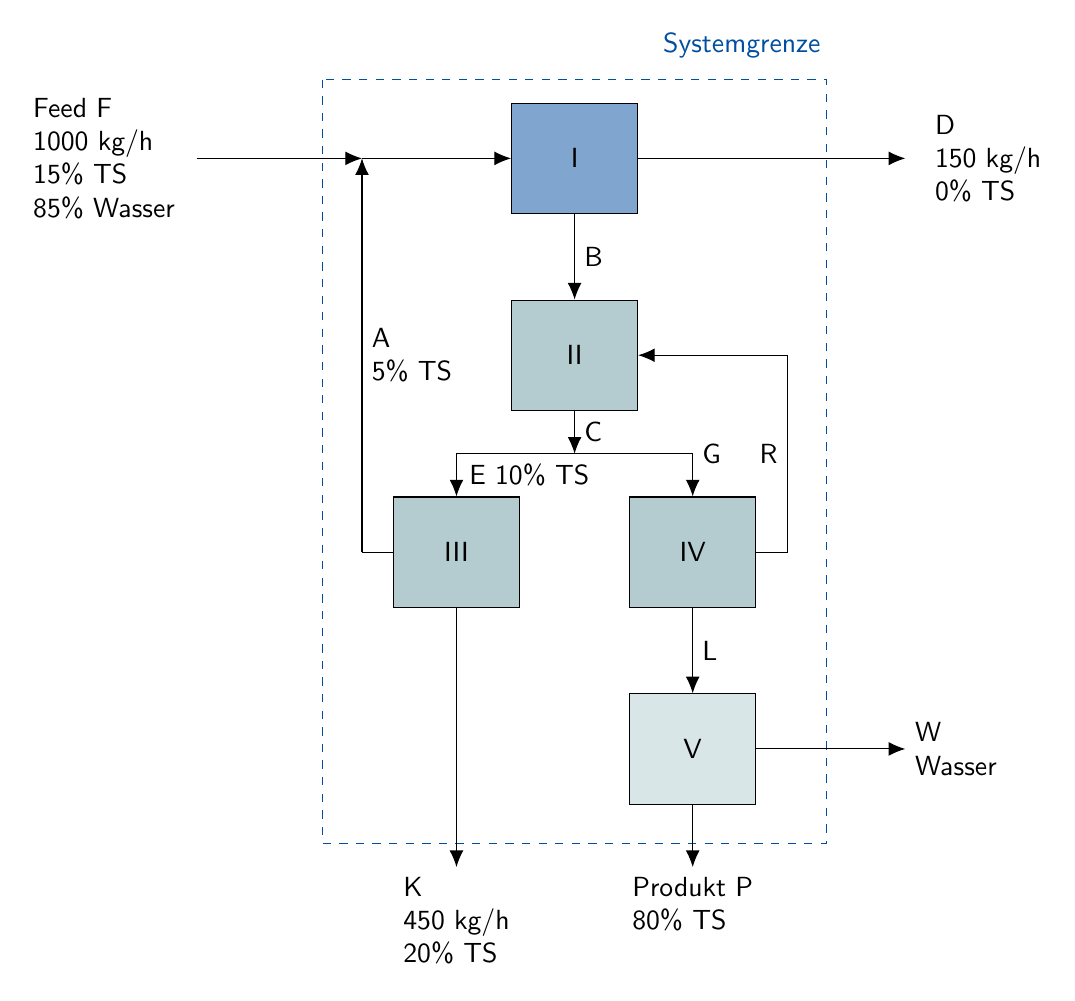
\begin{tikzpicture}[font=\sffamily, >={Latex[length=6pt, width=5pt]}]

    % --- Definition der Stile für die Blöcke ---
    \tikzset{
        block/.style={rectangle, draw=black, minimum width=1.6cm, minimum height=1.4cm, align=center},
		blaublock/.style={block, fill=uniblau!50},
        grayblock/.style={block, fill=miugray!50},
        redblock/.style={block, fill=miugray}
    }

    % --- Positionierung der Blöcke ---
    \node[blaublock] (I)   at (0, 0)      {I};
    \node[redblock]  (II)  at (0, -2.5)   {II};
    \node[redblock]  (III) at (-1.5, -5.0){III};
    \node[redblock]  (IV)  at (1.5, -5.0) {IV};
    \node[grayblock] (V)   at (1.5, -7.5) {V};

    % --- Systemgrenze (gestrichelte Linie) ---
    \draw[dashed, semithick, uniblau] (-3.2, 1) rectangle (3.2, -8.7);
    \node[above left, inner sep=2pt] at (3.2, 1.2) {\color{uniblau}Systemgrenze};

    % --- Stoffströme (Pfeile & Beschriftungen) ---
    
    % Feed F
    \draw[->] (-4.8, 0) -- (-2.7, 0);
    \draw[->] (-2.7, 0) -- (I.west);
    \node[left, align=left, inner sep=2pt] at (-5, 0) {Feed F \\ 1000 kg/h\\15\% TS\\85\% Wasser};

    % Stream D
    \draw[->] (I.east) -- (4.2, 0);
    \node[right, align=left, inner sep=2pt] at (4.5, 0) {D \\ 150 kg/h\\0\% TS};

    % Stream B
    \draw[->] (I.south) -- (II.north) node[midway, right] {B};

    % Stream C, E und G (Aufteilung)
    \draw[->]  (II.south) -- (0, -3.75) node[midway, right] {C};
    \draw[-]  (0, -3.75) -- (-1.5, -3.75) node[midway, below,xshift=5pt] {E 10\% TS};
    \draw[->] (-1.5, -3.75) -- (III.north);
    \draw[-]  (0, -3.75) -- (1.5, -3.75) node[right] {G};
    \draw[->] (1.5, -3.75) -- (IV.north);

    % Stream A (Rückführung)
    \draw[-]  (III.west) -- (-2.7, -5.0);
    \draw[->] (-2.7, -5.0) -- (-2.7, 0);
    \node[right, align=left] at (-2.7, -2.5) {A\\5\% TS};

    % Stream R (Rückführung)
    \draw[-]  (IV.east) -- (2.7, -5.0) -- (2.7, -2.5);
    \draw[->] (2.7, -2.5) -- (II.east);
    \node[left] at (2.7, -3.75) {R};

    % Stream L
    \draw[->] (IV.south) -- (V.north) node[midway, right] {L};

    % Stream K
    \draw[->] (III.south) -- (-1.5, -9.0) node[below, align=left] {K\\450 kg/h\\20\% TS};

    % Stream Product P
    \draw[->] (V.south) -- (1.5, -9.0) node[below, align=left] {Produkt P\\80\% TS};

    % Stream W
    \draw[->] (V.east) -- (4.2, -7.5) node[right, align=left] {W\\Wasser};

\end{tikzpicture}
}

\caption{Schematische Darstellung des Herstellungsprozesses. Abgeändert nach Singh und Heldman.}
\label{masse}
\end{figure}
\end{minipage}%
%\antwort{
%Produkt $P$:
%\begin{align*}
%F = D + W + K + P
%\end{align*}
%Für die Trockensubstanz gilt:
%\begin{align*}
%0,1 F &=  0 D + 0 W +0,2 K + 0,8 P \\
%0,1 F &=  0 + 0 +0,2 \cdot 450 + 0,8 P \\
%150 &= 90 + 0,8 P \\
%P &= 75 ~\text{kg/h}
%\end{align*}
%Rücklauf $A$:
%\begin{align*}
%E &= A + K \\
%0,1 E &= 0,05 A + 0,2 K \\
%0,1 (A+K) &= 0,05 A + 90 \\ 
%0,1 + 45 &= 0,05 A + 90 \\
%0,05 A &= 45 \\
%A &= 900 ~\text{kg/h}\\ \\
%E &= 1.350 ~\text{kg/h}
%\end{align*}
%}


\end{frame}







\begin{frame}
\begin{center}
\large Vielen Dank fürs Zuhören!
\par \normalsize ... und bis nächste Woche :)
\end{center}


\end{frame}



\end{document}
